\chapter{Background and related work}\label{ch:2}

\section{Raven's matrices and the three datasets}\label{sec:2.1}

\textbf{The format.} A Raven's Progressive Matrix, in its best-known form, is a three-by-three grid of panels with the last one missing. The figures change along the rows by rules the solver has to find, and the answer is chosen from eight candidates (\citealp{raven1938progressive}).

\textbf{RAVEN.} \citet{zhang2019raven} generate such puzzles by program. A puzzle has one of seven layouts: a single centred object, a 2×2 grid, a 3×3 grid, two objects side by side (left-right), two objects one above the other (up-down), one object inside another (in-out), and a 2×2 grid inside an object (in-out grid). The last four layouts have two \emph{components}, each with its own rules. Every object has a type, a size and a colour, with 5, 6 and 10 values, and a grid component also has the number of its objects and their positions. Each attribute follows one of four rules along every row:

\begin{center}\small
\begin{tabularx}{\linewidth}{@{}lY@{}}
\toprule
rule & a row (a, b, c) satisfies \\
\midrule
Constant & a = b = c \\
Progression & b − a = c − b, a fixed step of ±1 or ±2 \\
Arithmetic & c = a + b or c = a − b; on positions, the union or difference of the occupied slots \\
Distribute Three & the three panels hold three fixed values, in a different order in each row \\
\bottomrule
\end{tabularx}
\end{center}

The object's orientation follows no rule and acts as a distractor.

\textbf{I-RAVEN.} RAVEN builds each wrong candidate by changing one attribute of the answer. The answer is then the candidate that shares the most attribute values with the others, and a model can find it without looking at the matrix. \citet{hu2021stratified} showed this and regenerated the candidates so that the vote is balanced. In our own check, a model given only the eight candidates scores 90–100\% on RAVEN and is at chance on I-RAVEN (Chapter~\ref{ch:4}). All I-RAVEN experiments here use 10,000 puzzles per layout.

\textbf{I-RAVEN-X.} \citet{hersche2024towards} extend the single-object layout in two directions: rows of n panels instead of three, and values from 0 to m − 1, with m up to 1,000, instead of about ten values. Arithmetic then sums or subtracts n − 1 operands, and a model that stores sums has far more of them to store. I-RAVEN-X has no images; a puzzle is its attribute values. The generator's Distribute rule can also draw m itself, so the data hold values from 0 to m, and we name the datasets by that range: rows of 3 with values 0–10, and rows of 10 with values 0–50, 0–100 and 0–1,000. Figures~\ref{fig:iraven_puzzle} and \ref{fig:iravenx_puzzle} show a puzzle from each.

\begin{figure}[tbp]
\centering
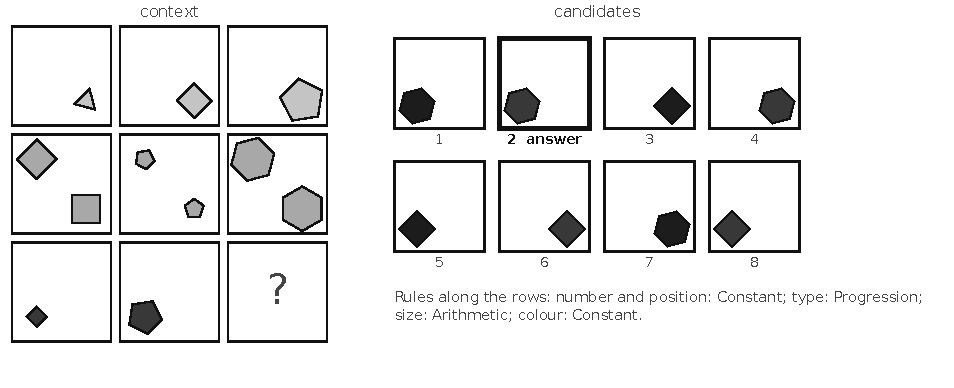
\includegraphics[width=\linewidth]{figures/iraven_puzzle}
\caption{An I-RAVEN puzzle from the distribute-four layout (training puzzle 67), drawn from its XML attributes. Along the rows, number and position follow Constant, type Progression, size Arithmetic and colour Constant. The answer is candidate 2.}\label{fig:iraven_puzzle}
\end{figure}

\begin{figure}[tbp]
\centering
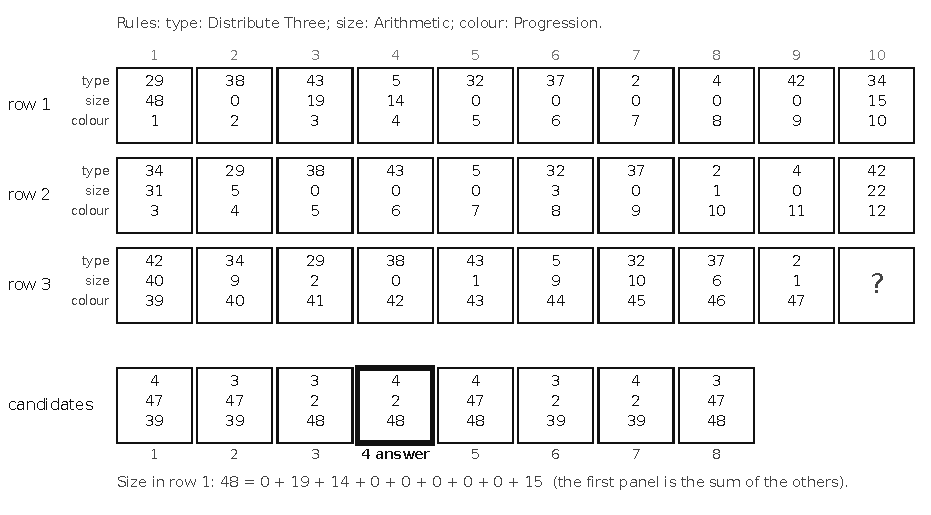
\includegraphics[width=\linewidth]{figures/iravenx_puzzle}
\caption{An I-RAVEN-X puzzle with rows of ten and values 0–50 (training puzzle 3): the last three rows of its 10 × 10 matrix, one object per panel, given as its type, size and colour values. Type follows Distribute Three, size Arithmetic and colour Progression. The answer is candidate 4.}\label{fig:iravenx_puzzle}
\end{figure}

\textbf{What generated puzzles are not.} The tests people take consist of a few dozen hand-made items, ordered from easy to hard, with no training set. The generated datasets keep the format and part of the rule list. In the RAVEN family the rules run along rows only, the list of attributes is fixed, and training and test puzzles come from one program. We measured how much depends on the row direction: after transposing an I-RAVEN matrix, 3\% of Progression instances and 1\% of Arithmetic instances still satisfy their rule, against 100\% for Distribute Three. \citet{barrett2018measuring} themselves call their generated task a different problem from the psychometric test. We therefore draw no conclusion about human reasoning from any number in this thesis, and return to what the generator contributes in Chapter~\ref{ch:8}.

\section{Graph neural networks}\label{sec:2.2}

A graph neural network keeps a vector for every node of a graph and updates it in rounds: each node collects messages from its neighbours, combines them with an operation that does not depend on their order, such as a sum or a mean, and passes the result through a learned function (\citealp{zhou2020graph}). The same functions serve every node and every edge. Two consequences matter here.

First, the network accepts graphs of any size, because its weights belong to the update rule and not to particular nodes. Second, renumbering the nodes changes nothing: the output of a node moves with the node. This permutation symmetry is the one symmetry every graph network has by construction. \citet{battaglia2018relational} describe the general point: an architecture expresses assumptions about the data, which they call relational inductive biases, and a graph network assumes that entities and their relations matter and their order does not.

What a plain graph network does not decide is everything else: which things are nodes, which edges exist, and which labels the nodes carry. A label such as ``row 1'' or ``the left component'', given to a node as an input feature, lets the network treat that row or component differently from the others. Chapter~\ref{ch:4} uses this. Two of our baselines are graph networks on the same graph, and differ only in whether nodes carry such absolute labels.

Edges join two nodes. A relation among three things, such as u + w = v among three numbers, is a hyperedge, and a network that passes messages along pairs has to be extended to use it.

\section{Lifted relational neural networks}\label{sec:2.3}

Lifted relational neural networks (\citealp{sourek2018lifted}, 2021) describe a model as a \emph{template}: a set of rules in the style of logic programming, with weights attached. A rule such as

\begin{Verbatim}[fontsize=\small,breaklines]
h(X) :- w1 : h(Y), w2 : edge(Y, X)
\end{Verbatim}

says how the value of \texttt{h} at any X is computed from the values at every Y joined to it. The variables stand for any constant. A \emph{sample} supplies the constants and the facts about them: the objects of one puzzle, their attributes, the panels they sit in.

\textbf{Grounding.} For each sample, the template and the facts are grounded: every way of substituting the sample's constants for a rule's variables that makes the rule's body derivable becomes one copy of the rule. The copies form a computation graph, with a neuron for each fact, each ground rule body, each aggregation over the bodies that share a head, and each derived atom (\citealp[Section 3.2]{sourek2021beyond}). A different sample gives a different network. The weights do not change: in the authors' words, they are shared ``in a scheme determined by the lifted structure of the template''. Variables that occur only in the body of a rule are aggregated over, which corresponds to quantifying over them. Figure~\ref{fig:grounding} shows one template grounded on two puzzles.

\begin{figure}[tbp]
\centering
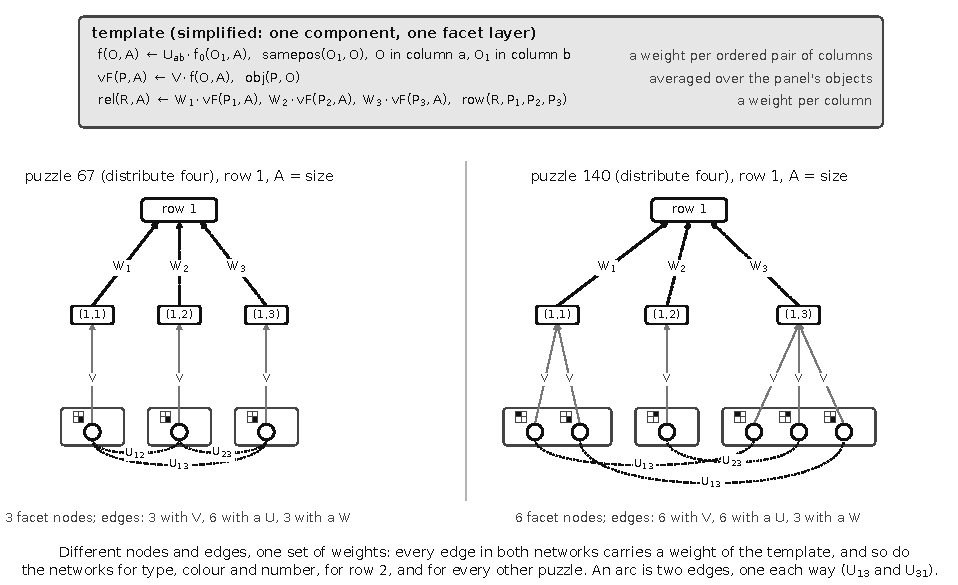
\includegraphics[width=\linewidth]{figures/grounding}
\caption{One template grounded on two puzzles (the size attribute in row 1 of each, with one facet layer). The two ground networks have different nodes and edges, but every edge carries one of the template's weights: V from a facet to its panel, W1 to W3 from the panels to the row, and U\_ab between objects at the same position in columns a and b.}\label{fig:grounding}
\end{figure}

\textbf{Relation to graph networks.} A message-passing layer is one such rule over \texttt{edge} facts, and \citet{sourek2021beyond} reproduce standard graph networks as templates. Templates go further in three ways that this thesis uses: rules over relations of any arity, so a three-way relation is as natural as an edge; rules that derive new relations from the facts before any learning takes place; and recursive rules, which unfold to whatever depth the sample's structure has. The authors list attention and gating as constructs that do not fit naturally.

\textbf{PyNeuraLogic} is the Python front end of the NeuraLogic engine. All our relational models are written in it and trained with its own optimizer, on CPU. The engine grounds each puzzle once and keeps the ground networks in memory, which sets the cost reported in Chapter~\ref{ch:5}.

The property this thesis builds on is the sentence quoted above. Chapter~\ref{ch:3} turns it into a theorem: a template cannot tell apart two constants that it does not name, so its output is unchanged by any renaming of such constants that maps the sample's facts onto themselves.

\section{Symmetry as inductive bias}\label{sec:2.4}

\textbf{Bias is necessary.} A learner that prefers no hypothesis over another cannot generalise beyond its training examples (\citealp{mitchell1980need}), and averaged over all problems no learner beats another (\citealp{wolpert1996lack}). An advantage always comes from an assumption that fits the problem. The open question is which assumptions to make, and the field disagrees on how many: \citet{sutton2019bitter} argues that general methods with more computation have overtaken hand-built knowledge again and again, while \citet{marcus2018deep} and \citet{lake2017building} argue that objects, relations and compositional structure have to be built in.

\textbf{Symmetry.} Let a group G act on the inputs of a function f. The function is \emph{invariant} if f(g·x) = f(x) for every g in G, and \emph{equivariant} if f(g·x) = g·f(x), where G also acts on the outputs. A model has a symmetry \emph{built in} when this holds for every setting of its weights, and has merely \emph{learned} it when it holds, approximately, after training. Geometric deep learning (\citealp{bronstein2021geometric}) reads the successful architectures this way: convolutional networks are equivariant to translations, group convolutions extend this to other groups (\citealp{cohen2016group}), networks on sets are invariant or equivariant to permutations (\citealp{zaheer2017deep}), as graph networks are (Section~\ref{sec:2.2}), and the architecture follows from the choice of domain and group.

\textbf{Symmetry is weight sharing.} \citet{ravanbakhsh2017equivariance} show that a layer is equivariant to a permutation group exactly when its weights are tied along the orbits of the group, and \citet{kondor2018generalization} that a layer equivariant to a compact group must be a convolution over that group. Chapter~\ref{ch:3} proves the lifted counterpart: in a template the tying is done by variables, and the group is whatever the unnamed constants and the background facts leave free.

\textbf{What a symmetry is worth.} A symmetry that the target function shares shrinks the set of functions the model can represent without removing the target, so fewer examples are needed. \citet{sokolic2017generalization} bound the generalisation error of an invariant classifier through the covering number of the base space that is left when the transformations are factored out. For T transformations that keep the transformed copies apart, this number is up to T times smaller, so the bound is up to √T smaller, which is the bound of a non-invariant classifier trained on up to T times as many examples. \citet{elesedy2021provably} prove a strict generalisation benefit for equivariant models (for squared loss and a symmetric input distribution, computed exactly for linear models), and \citet{bietti2021sample} and \citet{tahmasebi2023exact} give sample-complexity gains proportional to the size of the group for kernel methods, once the sample is large enough. These results say that the gain grows with the group. They are stated for function classes and data distributions in general; they do not say what a particular symmetry is worth on a particular rule, which is what we count in Chapter~\ref{ch:3}, and, for the components of Chapter~\ref{ch:6}, in training puzzles (Section~\ref{sec:6.2}).

\textbf{What a wrong symmetry costs.} A model can also have a symmetry that the task lacks. \citet{wang2023general} sort this into three cases, by what the symmetry does to the data. Equivariance is \emph{correct} where the transformed input also occurs in the data and has the transformed label, \emph{incorrect} where the transformed input also occurs in the data but with a different label, and \emph{extrinsic} where the transformed input lies outside the data distribution. For incorrect equivariance they prove a lower bound on the error, computed orbit by orbit: an invariant model gives every input of an orbit the same label, so on each orbit it loses at least the probability mass that does not carry the orbit's commonest label (their Theorem 4.3). The bound needs no assumption that the data's distribution is symmetric, and some invariant model attains it. Their earlier paper showed that extrinsic equivariance can help (\citealp{wang2023surprising}); this one shows that it can also hurt (their Section 5). \citet{petrache2023approximation} analyse the trade-off between the approximation error of a misspecified symmetry and its generalisation gain. The three kinds of symmetry in our Chapter~\ref{ch:3} (data symmetry, out of support, conflicting) are these three cases, reached from the generator's side, and the ceiling we compute for a conflicting symmetry is their bound evaluated on a rule's table. What we add is the other half of the count, the data a correct symmetry saves, and matched experiments in which both halves are predicted before training. Softer forms exist as well: a model can be given a preference for a symmetry and not a constraint (\citealp{finzi2021residual}; \citealp{wang2022approximately}). Chapter~\ref{ch:6} has a small result of that kind, where a model that shares all its weights but is not exactly invariant does as well as the exactly invariant one.

\textbf{Shortcuts.} A model without the right constraint may fit the training data by a rule that holds only there (\citealp{geirhos2020shortcut}). RAVEN's candidate sets are one example. Chapter~\ref{ch:6} shows another, in which a model that is allowed to tell panels apart learns one rule by the panel's address.

\textbf{Structure that matches the computation.} \citet{xu2020what} show that a network learns a task more easily when its structure mirrors the algorithm that solves it, and \citet{xu2021how} that a graph network's success in extrapolating algorithmic tasks relies on the task's non-linearities being built into the architecture or the features. Chapter~\ref{ch:7} gives a case: a model learns sums from a hundred puzzles once addition is available as a relation, and not at all without it.

\textbf{Values on a line without a zero.} A symmetry that Chapter~\ref{ch:7} turns on is the shift of all values by a constant. \citet{stevens1946theory} classifies scales by the transformations they survive: on an interval scale the zero is a convention, and only differences mean something. In geometric terms such values form an affine line, on which points can be subtracted but not added, and a weighted sum of points is defined without reference to an origin when the weights sum to one (\citealp[Lemma 2.2.1]{gallier2011geometric}). A rule c = pa + qb therefore survives a common shift exactly when p + q = 1. The midpoint of two values satisfies this and their sum does not.

\textbf{Priors and the measurement of skill.} \citet{chollet2019measure} argues that skill at a task can be bought with training data or with built-in knowledge, so a score is informative only together with both. He names the priors a fair test may assume, among them objects, elementary geometry, and small numbers with addition and subtraction (in his own benchmark, below about ten), and he counts generation from one fixed program as a weakness of a benchmark, since learning the program solves every task. RAVEN is such a benchmark. We use his terms in Chapter~\ref{ch:8} to sort our priors into those a person would bring to any such test and those read off the generator.

\section{Solvers of Raven's matrices}\label{sec:2.5}

\textbf{Black-box image models.} The first neural solvers map the images to an answer and are trained on the answer's index. WReN (\citealp{barrett2018measuring}) scores each candidate with a relation network over panel embeddings. \citet{zhuo2020solving}, the reference named in this thesis's assignment, give a ResNet the sixteen panels as one stack of images and train it on the answer's index. With ImageNet pre-training a ResNet-50 answers 86\% of RAVEN's test puzzles, above the human score that RAVEN reports, but it falls by 17 to 19 points when tested on layouts it was not trained on. Without answer labels, trained only on the assumption that the third row obeys the rules of the first two, a network reaches 28.5\%, against 12.5\% for guessing. Their results are on RAVEN, before its candidate shortcut was found. Later models add structure that matches the generator: CoPINet contrasts the candidates (\citealp{zhang2019learning}), SRAN encodes rows hierarchically (\citealp{hu2021stratified}), and SCL shares networks across objects, attributes and relations (\citealp{wu2020scattering}). Several of these are symmetry priors in our sense, and we credit them as such. All of them classify among the candidates. Reported accuracies on I-RAVEN reach about 98\%, but when \citet{malkinski2025airaven} retrained thirteen of these models under one protocol, most scored far lower: DRNet 90.9\% against a reported 97.6\%, SCL 83.4\% against 95.0\%, STSN 59.0\% against 95.7\%.

\textbf{Object-centric and graph models.} A second group first finds the objects and then reasons over them, which is the plan the assignment asks for. \citet{spratley2020closer} attend to objects before relating panels, \citet{wang2020abstract} build a multiplex graph over the objects of a puzzle, and \citet{mondal2023learning} combine slot attention with a transformer. Our facet model belongs here, with two differences: its graph has one node per attribute of an object, not per object, and it generates the answer.

\textbf{Neuro-symbolic models.} PrAE (\citealp{zhang2021abstract}) recognises the objects of each panel as probability distributions over attribute values, infers which of the generator's rules each attribute follows, executes the rule to predict the answer's attributes, and picks the nearest candidate. The rules are given. It is trained on the answer's index, through a choice among the eight candidates, with the rules of each training puzzle as an auxiliary target. This is the closest precedent for our task of generating the answer and then matching, and for the symbolic reference models of Chapter~\ref{ch:4}. ALANS (\citealp{zhang2022learning}) removes the given rules by representing values as matrices and learning operators on them. NVSA (\citealp{hersche2023neuro}) represents attributes as high-dimensional vectors and writes each rule as an expression in vector-symbolic algebra; ARLC (\citealp{camposampiero2024towards}) learns such expressions from data. In these models addition is an operation of the representation, so they compare with our models that are given addition, not with those that have to learn sums (Chapter~\ref{ch:7}).

\textbf{Language models.} Given the attribute values as text, large language models solve many of these puzzles without training on them. \citet{hersche2024towards} report that GPT-4, given the attribute values as text, answers 93\% of I-RAVEN's centre puzzles and 77–82\% of I-RAVEN-X puzzles with rows of 10, and that on Arithmetic at range 50 it reaches 30\% where the learned ARLC reaches 82\%.

\textbf{Arithmetic in neural networks.} Networks that are not given addition learn it poorly. \citet{trask2018neural} find that networks trained on sums fail outside the trained range and describe the failure as memorisation. Small transformers trained on modular addition first memorise and, much later, generalise (\citealp{power2022grokking}), by representing each number as an angle so that adding becomes rotating (\citealp{nanda2023progress}). \citet{mohamadi2024why} prove that a permutation-equivariant kernel method, which is how a network behaves early in training, must see a constant fraction of the table of modular addition before it generalises. That is the situation of a model with separate weights for every value, and in Chapter~\ref{ch:7} such a model tracks a learner that only memorises.

\section{Where this thesis stands}\label{sec:2.6}

Three things separate this work from the solvers above.

\begin{itemize}
\item \textbf{The question is the price of a prior, not the score.} The models above each add structure and report accuracy. We take one model family and add or remove one symmetry at a time, at several amounts of training data, and compare each result with a number computed before training.
\item \textbf{The symmetry is declared.} In a template a symmetry is the absence of a name, and one theorem covers every symmetry built this way. The architectures above are each engineered for their symmetry, and each needs its own argument.
\item \textbf{The answer is generated and the candidates are never seen}, in training or as input. Only PrAE and its successors also generate the answer before matching, and they are given the rules or the operations; PrAE is still trained through a choice among the candidates.
\end{itemize}
